\documentclass[border=4pt,dvisvgm]{standalone}
\usepackage{tikz}
\usetikzlibrary{arrows.meta,positioning,shapes.geometric,fit,calc,backgrounds}
\begin{document}
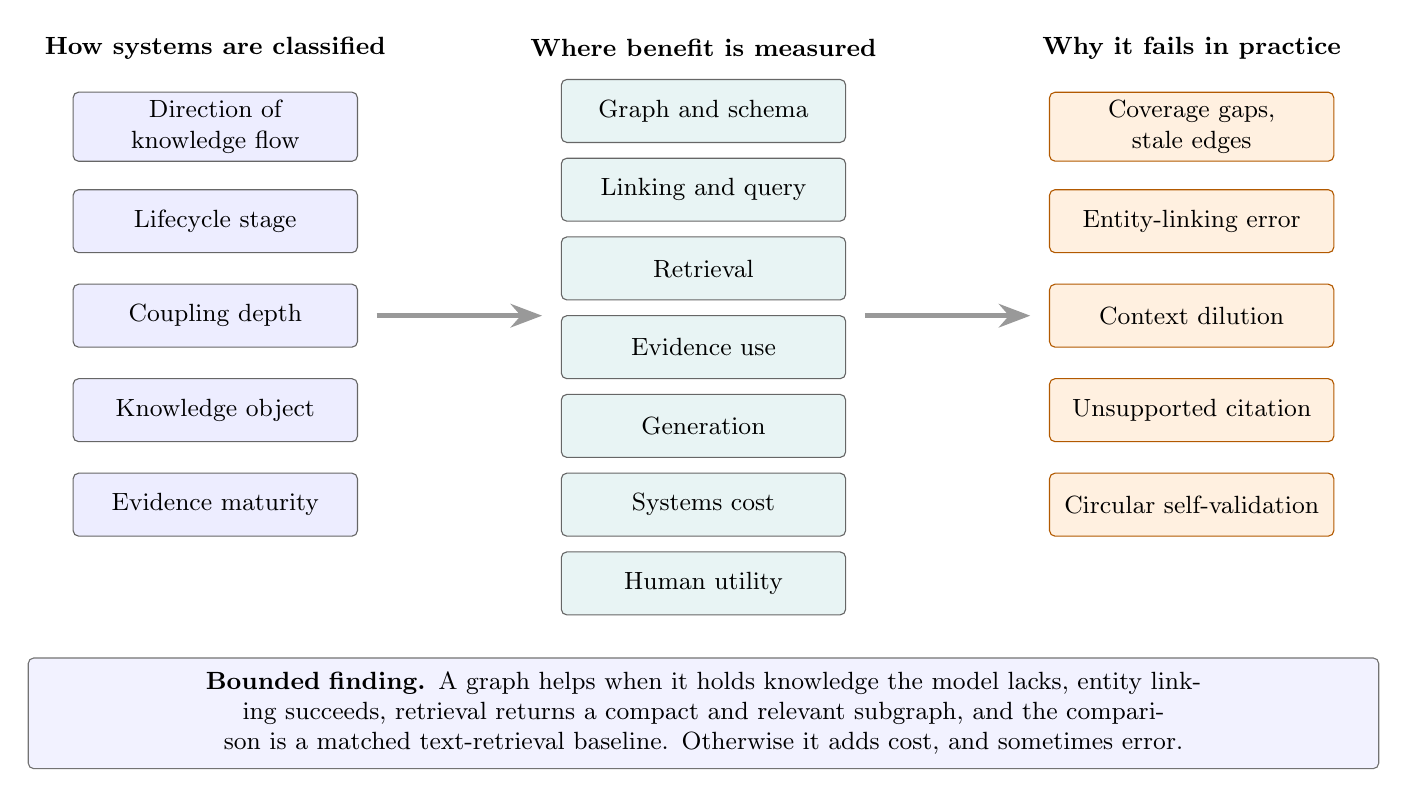
\begin{tikzpicture}[
  font=\small,
  hdr/.style={font=\small\bfseries, align=center},
  ax/.style={draw=black!60, rounded corners=2pt, fill=blue!7,
             text width=34mm, align=center, minimum height=8mm, inner sep=3pt},
  lay/.style={draw=black!60, rounded corners=2pt, fill=teal!9,
              text width=34mm, align=center, minimum height=8mm, inner sep=3pt},
  fail/.style={draw=orange!70!black, rounded corners=2pt, fill=orange!12,
               text width=34mm, align=center, minimum height=8mm, inner sep=3pt},
  big/.style={-{Stealth[length=4mm]}, line width=1.6pt, draw=black!40}
]

% ---- column 1: five classification axes
\node[hdr] (h1) at (0,1.35) {How systems are classified};
\node[ax] (a1) at (0,0.35)   {Direction of knowledge flow};
\node[ax] (a2) at (0,-0.85)  {Lifecycle stage};
\node[ax] (a3) at (0,-2.05)  {Coupling depth};
\node[ax] (a4) at (0,-3.25)  {Knowledge object};
\node[ax] (a5) at (0,-4.45)  {Evidence maturity};

% ---- column 2: seven evaluation layers
\node[hdr] (h2) at (6.2,1.35) {Where benefit is measured};
\node[lay] (l1) at (6.2,0.55)   {Graph and schema};
\node[lay] (l2) at (6.2,-0.45)  {Linking and query};
\node[lay] (l3) at (6.2,-1.45)  {Retrieval};
\node[lay] (l4) at (6.2,-2.45)  {Evidence use};
\node[lay] (l5) at (6.2,-3.45)  {Generation};
\node[lay] (l6) at (6.2,-4.45)  {Systems cost};
\node[lay] (l7) at (6.2,-5.45)  {Human utility};

% ---- column 3: failure modes
\node[hdr] (h3) at (12.4,1.35) {Why it fails in practice};
\node[fail] (f1) at (12.4,0.35)  {Coverage gaps, stale edges};
\node[fail] (f2) at (12.4,-0.85) {Entity-linking error};
\node[fail] (f3) at (12.4,-2.05) {Context dilution};
\node[fail] (f4) at (12.4,-3.25) {Unsupported citation};
\node[fail] (f5) at (12.4,-4.45) {Circular self-validation};

% ---- flow arrows between columns
\draw[big] (2.05,-2.05) -- (4.15,-2.05);
\draw[big] (8.25,-2.05) -- (10.35,-2.05);

% ---- conclusion strip
\node[draw=black!55, fill=blue!5, rounded corners=2pt, text width=168mm,
      align=center, inner sep=5pt, font=\small] at (6.2,-7.1)
  {\textbf{Bounded finding.} A graph helps when it holds knowledge the model lacks, entity linking
   succeeds, retrieval returns a compact and relevant subgraph, and the comparison is a matched
   text-retrieval baseline. Otherwise it adds cost, and sometimes error.};
\end{tikzpicture}%
\end{document}
